\documentclass{report}

\newcommand{\Alpha}{A}

\newcommand{\project}{DotMachine}
\newcommand{\maxX}{28}
\newcommand{\maxY}{11}
\newcommand{\maxXY}{\number\numexpr\maxX*\maxY\relax}
\newcommand{\maxFace}{2}
\newcommand{\maxFaceMulXY}{\left(\maxFace\times{\maxXY}\right)}

\newcommand{\violet}{\colorbox{violet!10}}
\newcommand{\bonus}{\violet}

\usepackage[french]{babel}
\usepackage[T1]{fontenc}
\usepackage[utf8]{inputenc}
\usepackage{fontspec}
\usepackage[a4paper]{geometry}
\usepackage{scrextend}
\usepackage{listings}
\usepackage[hidelinks,unicode=true]{hyperref}
\usepackage[pgf]{dot2texi}
\usepackage{pgf}
\usepackage{tikz}
\usepackage{fancyhdr}
\usepackage{sectsty}
\usepackage{titlesec}
\usepackage{csquotes}
\usepackage{hyperref}
\usepackage{keystroke}
\usepackage{booktabs}
\usepackage{color, colortbl}
\usepackage[labelformat=empty]{caption}
\usepackage{framed}
\usepackage{amsmath}
\usepackage[linguistics]{forest}
\usepackage{adjustbox}

\setcounter{tocdepth}{4}
\setcounter{secnumdepth}{4}

\hypersetup{
  colorlinks = true,
  linkcolor = blue,
  urlcolor = blue,
}

\usetikzlibrary{automata, shapes, arrows, snakes, matrix, positioning}

\pagestyle{fancy}

\fancyhf{}
\lhead{\leftmark}
\rhead{\rightmark}
\rfoot{\thepage}

\setmainfont[
	Path = assets/fonts/,
	Extension = .ttf,
	Ligatures = TeX,
	Scale = MatchLowercase,
]{sazanami-mincho}

\setsansfont[
	Path = assets/fonts/,
	Extension = .ttf,
	Ligatures = TeX,
	Scale = MatchLowercase,
]{sazanami-gothic}

\title{}

\author{
   adjivas
   \and
   jb
}

\date{}

\begin{document}

\begin{titlepage}
    \vspace*{\stretch{1.0}}
    \begin{center}
        \huge \textbf{TETRIS} \\
        \vspace*{\stretch{0.09}}
        \large \textbf{DOT} \\
        \vspace*{\stretch{0.05}}
        \Huge \textbf{MACHINE} \\
    \end{center}
\vspace*{\stretch{2.0}}
\end{titlepage}

\tableofcontents

\titleformat{\chapter}[display]
  {\Huge}
  {\filleft\texttt{\chaptertitlename} \Huge\thechapter}
  {0ex}
  {\filleft}
  [\titlerule]

\chapter{Software}

Le projet \project{} est un Tetris multijoueurs sur girouette a pastille. \\*
\noindent \project{} est composé de deux cartes reliées en Uart. Chacune est dotée d'une alimentation avec interupteur marche/arrêt et de d'une manettes PSX en entre. D'un bipeur et d'un afficheurs en sortie.
\begin{figure}[!ht]
    \begin{center}
	\begin{tikzpicture}[
	    >=stealth,
	    every node/.style={shape=rectangle,draw,rounded corners},
	]
	    \node (l1) {Manette};
	    \node (l2) [below =of l1]{Marche/Arrêt};
	    \node (m1) [right =of l1]{\project};
	    \node (r1) [right =of m1]{Afficheur};
	    \node (r2) [above right =of m1]{Bipeur};

	    \draw[->] (l1) to (m1);
	    \draw[->] (l2) to (m1);
	    \draw[->] (m1) to (r1);
	    \draw[->] (m1) to (r2);
	\end{tikzpicture}
    \end{center}
\end{figure}

\newpage
\section{Manette}

\begin{figure}[!ht]
    \begin{center}
        \begin{tikzpicture}
            \node[anchor=south west,inner sep=0] (image) at (0,0,0) {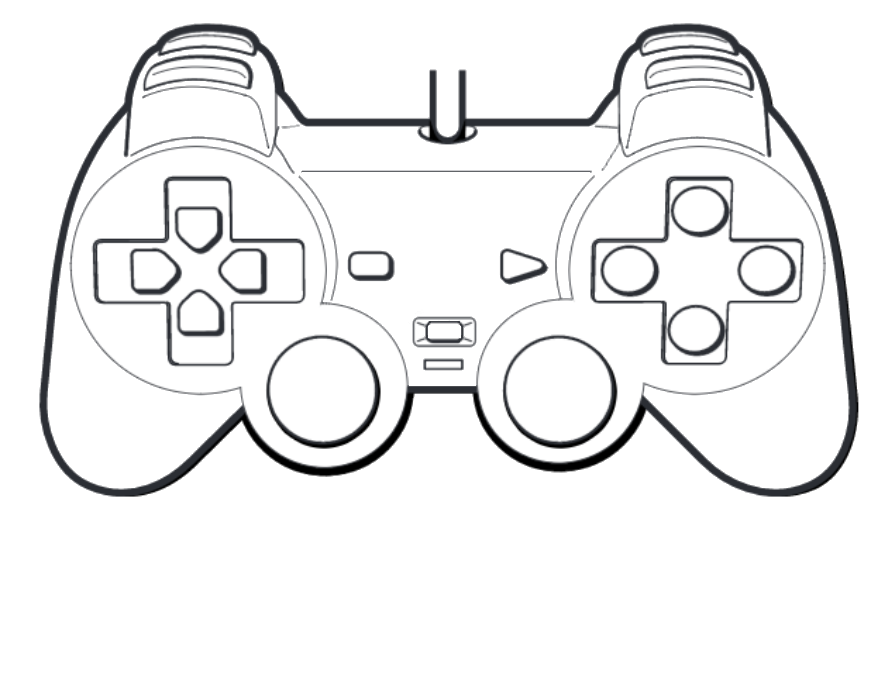
\includegraphics[scale=0.25]{assets/images/pad.png}};
            \begin{scope}[x={(image.south east)},y={(image.north west)}]

                % Select
                \draw[color=gray, *-] (0.58, 0.6) -- (0.58, 1) node[anchor=south] {menu};
                % Start
                \draw[color=gray, *-] (0.42, 0.6) -- (0.42, 1) node[anchor=south] {tetris};

                % L
                \draw[color=gray, *-] (0.25, 0.93) -- (0.25, 1) node[anchor=south] {son};
                \draw[color=gray, *-] (0.2, 0.90) -- (0, 0.90) -- (0, 1) node[anchor=south] {chute};

                % R
                %\draw[color=gray, *-] (0.75, 0.93) -- (0.75, 1) node[anchor=south] {};
                %\draw[color=gray, *-] (0.8, 0.90) -- (1, 0.90) -- (1, 1) node[anchor=south] {};

                % top
                \draw[color=gray, *-] (0.234, 0.674) -- (0, 0.674) -- (0, 0.79) -- (-0.1, 0.79) node[anchor=east] {rotation};
                % right
                \draw[color=gray, *-] (0.18, 0.605) -- (-0.1, 0.605) node[anchor=east] {gauche};
                % bottom
                \draw[color=gray, *-] (0.229, 0.55) -- (0.229, 0.445) -- (-0.1, 0.445) node[anchor=east] {bas};
                % left
                \draw[color=gray, *-] (0.28, 0.62) -- (0.28, 0.27) -- (-0.1, 0.27) node[anchor=east] {droite};

                % triangle
                \draw[color=gray, *-] (0.775, 0.69) -- (1, 0.69) -- (1, 0.79) -- (1.1, 0.79) node[anchor=west] {\bonus{rotation adverse}};
                % circle
                \draw[color=gray, *-] (0.852, 0.605) -- (1.1, 0.605) node[anchor=west] {\bonus{droite adverse}};
                % cross
                \draw[color=gray, *-] (0.78, 0.53) -- (0.78, 0.445) -- (1.1, 0.445) node[anchor=west] {\bonus{bas adverse}};
                % square
                \draw[color=gray, *-] (0.705, 0.62) -- (0.705, 0.275) -- (1.1, 0.275) node[anchor=west] {\bonus{gauche adverse}};
            \end{scope}
        \end{tikzpicture}
        \caption[Caption for LOF] {
	        \begin{tabular}{p{.15\textwidth}p{.15\textwidth}p{.65\textwidth}}
	            \toprule
	            \toprule
		        PSX & Clavier & Description \\
	            \midrule
                \keystroke{Select} & & Retourner au menu. \\
                \keystroke{Start} & & Lancer ou relancer une partie. \\
                \keystroke{L2} & & Active ou désactive le son. \\
                \keystroke{L1} & \End & Chuter la pièce. \\
                \UArrow{} & \UArrow{} & Tourner la pièce. \\
                \RArrow{} & \RArrow{} & Déplacer la pièce vers la droite. \\
                \LArrow{} & \LArrow{} & Déplacer la pièce vers la gauche. \\
                \DArrow{} & \DArrow{} & Déplacer la pièce vers le bas. \\
                \keystroke{Tl} & & Tourner la pièce adverse. \\
                \keystroke{Cl} & & Déplacer la pièce adverse vers la droite. \\
                \keystroke{Sr} & & Déplacer la pièce adverse vers la gauche. \\
                \keystroke{Cr} & & Déplacer la pièce adverse vers le bas. \\
	            \bottomrule
	        \end{tabular}
        }
    \end{center}
\end{figure}

\newpage
\section{Afficheur}

La girouette à pastilles \textit{IS213 ISSUE B} du constructeur \href{http://www.hanoverdisplays.com}{Hanover} comprend $\maxX \times \maxY$ pastilles, animees éléctromagnetiquement, de face respectivement jaune et noire.
\\
Selon la feuille technique \href{https://flipdots.com/wp-content/uploads/2016/10/electromagnetic_status_indicators.pdf}{AZ36}, une pastille mets 2 mili-seconde a chaniger son état.
\\
\begin{figure}[!ht]
    \begin{center}
	\begin{tikzpicture}[scale=0.3,rotate=90,transform shape]
	    \foreach \indexY in {1,...,\maxY} {
		\foreach \indexX in {1,...,\maxX} {
		    \pgfmathparse{int(mod(\indexX, 2))}
		    \pgfmathparse{random(0,1)}
		    \ifnum\pgfmathresult=0
			\draw node[fill = black, draw, regular polygon, regular polygon sides = 8, minimum size = 3em] at (\indexX, \indexY) {};
		    \else
			\draw node[fill = white, draw, regular polygon, regular polygon sides = 8, minimum size = 3em] at (\indexX, \indexY) {};
		    \fi
		}
	    }
	    \foreach \indexY in {3,...,\maxY} {
		    \foreach \indexX in {1,...,\maxX} {
		        \draw node[draw, rectangle, minimum width = 3em, minimum height = 3cm] at (\indexX, \indexY - 1) {};
		    }
	    }
	\end{tikzpicture}
	\caption[Caption for LOF]{IS213 ISSUE B}
    \end{center}
\end{figure}

\chapter{Hardware}

\begin{adjustbox}{max width=14.5cm}
    \begin{tikzpicture}[transform shape]
        \node (l1) [left =of l1] {
            $\begin{matrix}
                \hline\hline
                    Comment & LogicalDesignator & Ref fabricant & fournisseur & Ref fournisseur & Quantity
                \\ \hline
                    Buzzer & U10 & ABT-410-RC & Farnell & 1022402 & 2 \\
                    Conecteur alimentation & J7 & RAPC722X & Farnell & 1608727 & 2 \\
                    Conecteur limande 16 fils & J5, J6 & HTSS-108-02-L-D & Farnell & 1929447 & 4 \\
                    Conecteur limande 34 fils & J4 & HTSS-117-01-G-D & Farnell & 1930905 & 2 \\
                    Conecteur psx & J2 & 3041438 & Farnell & 3041438 & 2 \\
                    Connecteur uart & J3 & 3041360 & Farnell & 3041360 & 4 \\
                    Multiplexer ADG1606 & U4, U5, U6, U7 & ADG1606BRUZ & Farnell & 1827328 & 10 \\
                    PIC32MX170F256B-I/SO & U3 & PIC32MX170F256B-I/SO & Farnell & 2449077 & 2 \\
                    Porte NOT & U8, U9 & M74VHC1GT04DFT2G & Farnell & 2464475 & 4 \\
                    Program/Debug & J1 & 640456-6 & Farnell & 588611 & 2 \\
                    Regulateur tension & U2 & MIC2920A-3.3WS-TR & farnell & 2510013 & 2 \\
                    0.1uf & C1, C2, C4 & & & & 6 \\
                    10uf & C3, C9 & & & & 4 \\
                    1uF & C10 & & & & 2 \\
                    2.2uF & C5, C7 & & & & 4 \\
                    10k & R3 & & & & 2 \\
                    1K & R1 & & & & 2 \\
                    200r & R2 & & & & 2 \\
            \end{matrix}$
        };
        \node (m1) [below =of l1] {};
        \node (r1) [below left =of m1] {
            $\begin{matrix}
                \hline\hline
                    \multicolumn{2}{c}{version 1.0} 
                \\ \hline
                inverseur & U1 & LM2776DBVT & Farnell & 2498456 & 1 \\
            \end{matrix}$
        };
        \node (r2) [below right =of m1] {\bonus{
            $\begin{matrix}
                \hline\hline
                    \multicolumn{2}{c}{version 1.\pi} 
                \\ \hline
                    Mosfet P & U? & FQP7P06 & Farnell & 9846557 & 1 \\
                    Mosfet N & U? & FQP85N06 & Farnell & 9845739 & 1 \\
            \end{matrix}$
        }};
        \begin{scope}[very thick, -stealth]
    	    \draw[->] (m1) to (r1);
    	    \draw[->] (m1) to (r2);
    	\end{scope}
    \end{tikzpicture}
\end{adjustbox}

\newpage
\section{Version $1.0$}
\section{Version $1.\pi$}

\end{document}
